\documentclass[11pt]{article}

\usepackage[spanish,activeacute]{babel}
\usepackage[dvips]{graphicx}
\usepackage{color,graphpap}
\definecolor{gris}{cmyk}{0,0,0,0.5}

\begin{document}
\par 
Usando rotaciones cabmiando el origen de la rotaci'on.
\par 
\fbox{\parbox{2.4cm}{A sus pies, \emph{madmoiselle}.}}\quad \rotatebox[origin=lt]{-45}{\fbox{\parbox{2.4cm}{A sus pies, \emph{madmoiselle}.}}}

\par Usando rotacion y escalamaineto simult'aneamente.
\par 
\resizebox{2\width}{0.8\height}{\rotatebox{30}{\fbox{%
\parbox{5.5cm}{La b'usqueda de la verdad es m'as fascinante que su posesi'on. \rightline{Gothald Lessing}}}}}

\par Importando una gr'afica
\par La siguiente gr'afica es una 'util red:
\par 

\begin{center}
	\setlength{\unitlength}{1pt}
	\begin{picture}(250,80)
		\graphpaper(0,0)(250,80)
	\end{picture}
\end{center}
\vspace{1cm}
\par 

Yo puedo tambi'en introducir cosas en la gr'afica con el comando {\tt \textbackslash put($y$,$x$)\{objeto\}}, asi:
\begin{center}
\setlength{\unitlength}{2pt}
	\begin{picture}(150,50)
		{\color{gris}\graphpaper(0,0)(150,50)}
		\put(20,10){Ca'in}
		\put(60,30){Abel}
		\put(100,20){\Large Sans'on}
	\end{picture}
\end{center}



\begin{center}
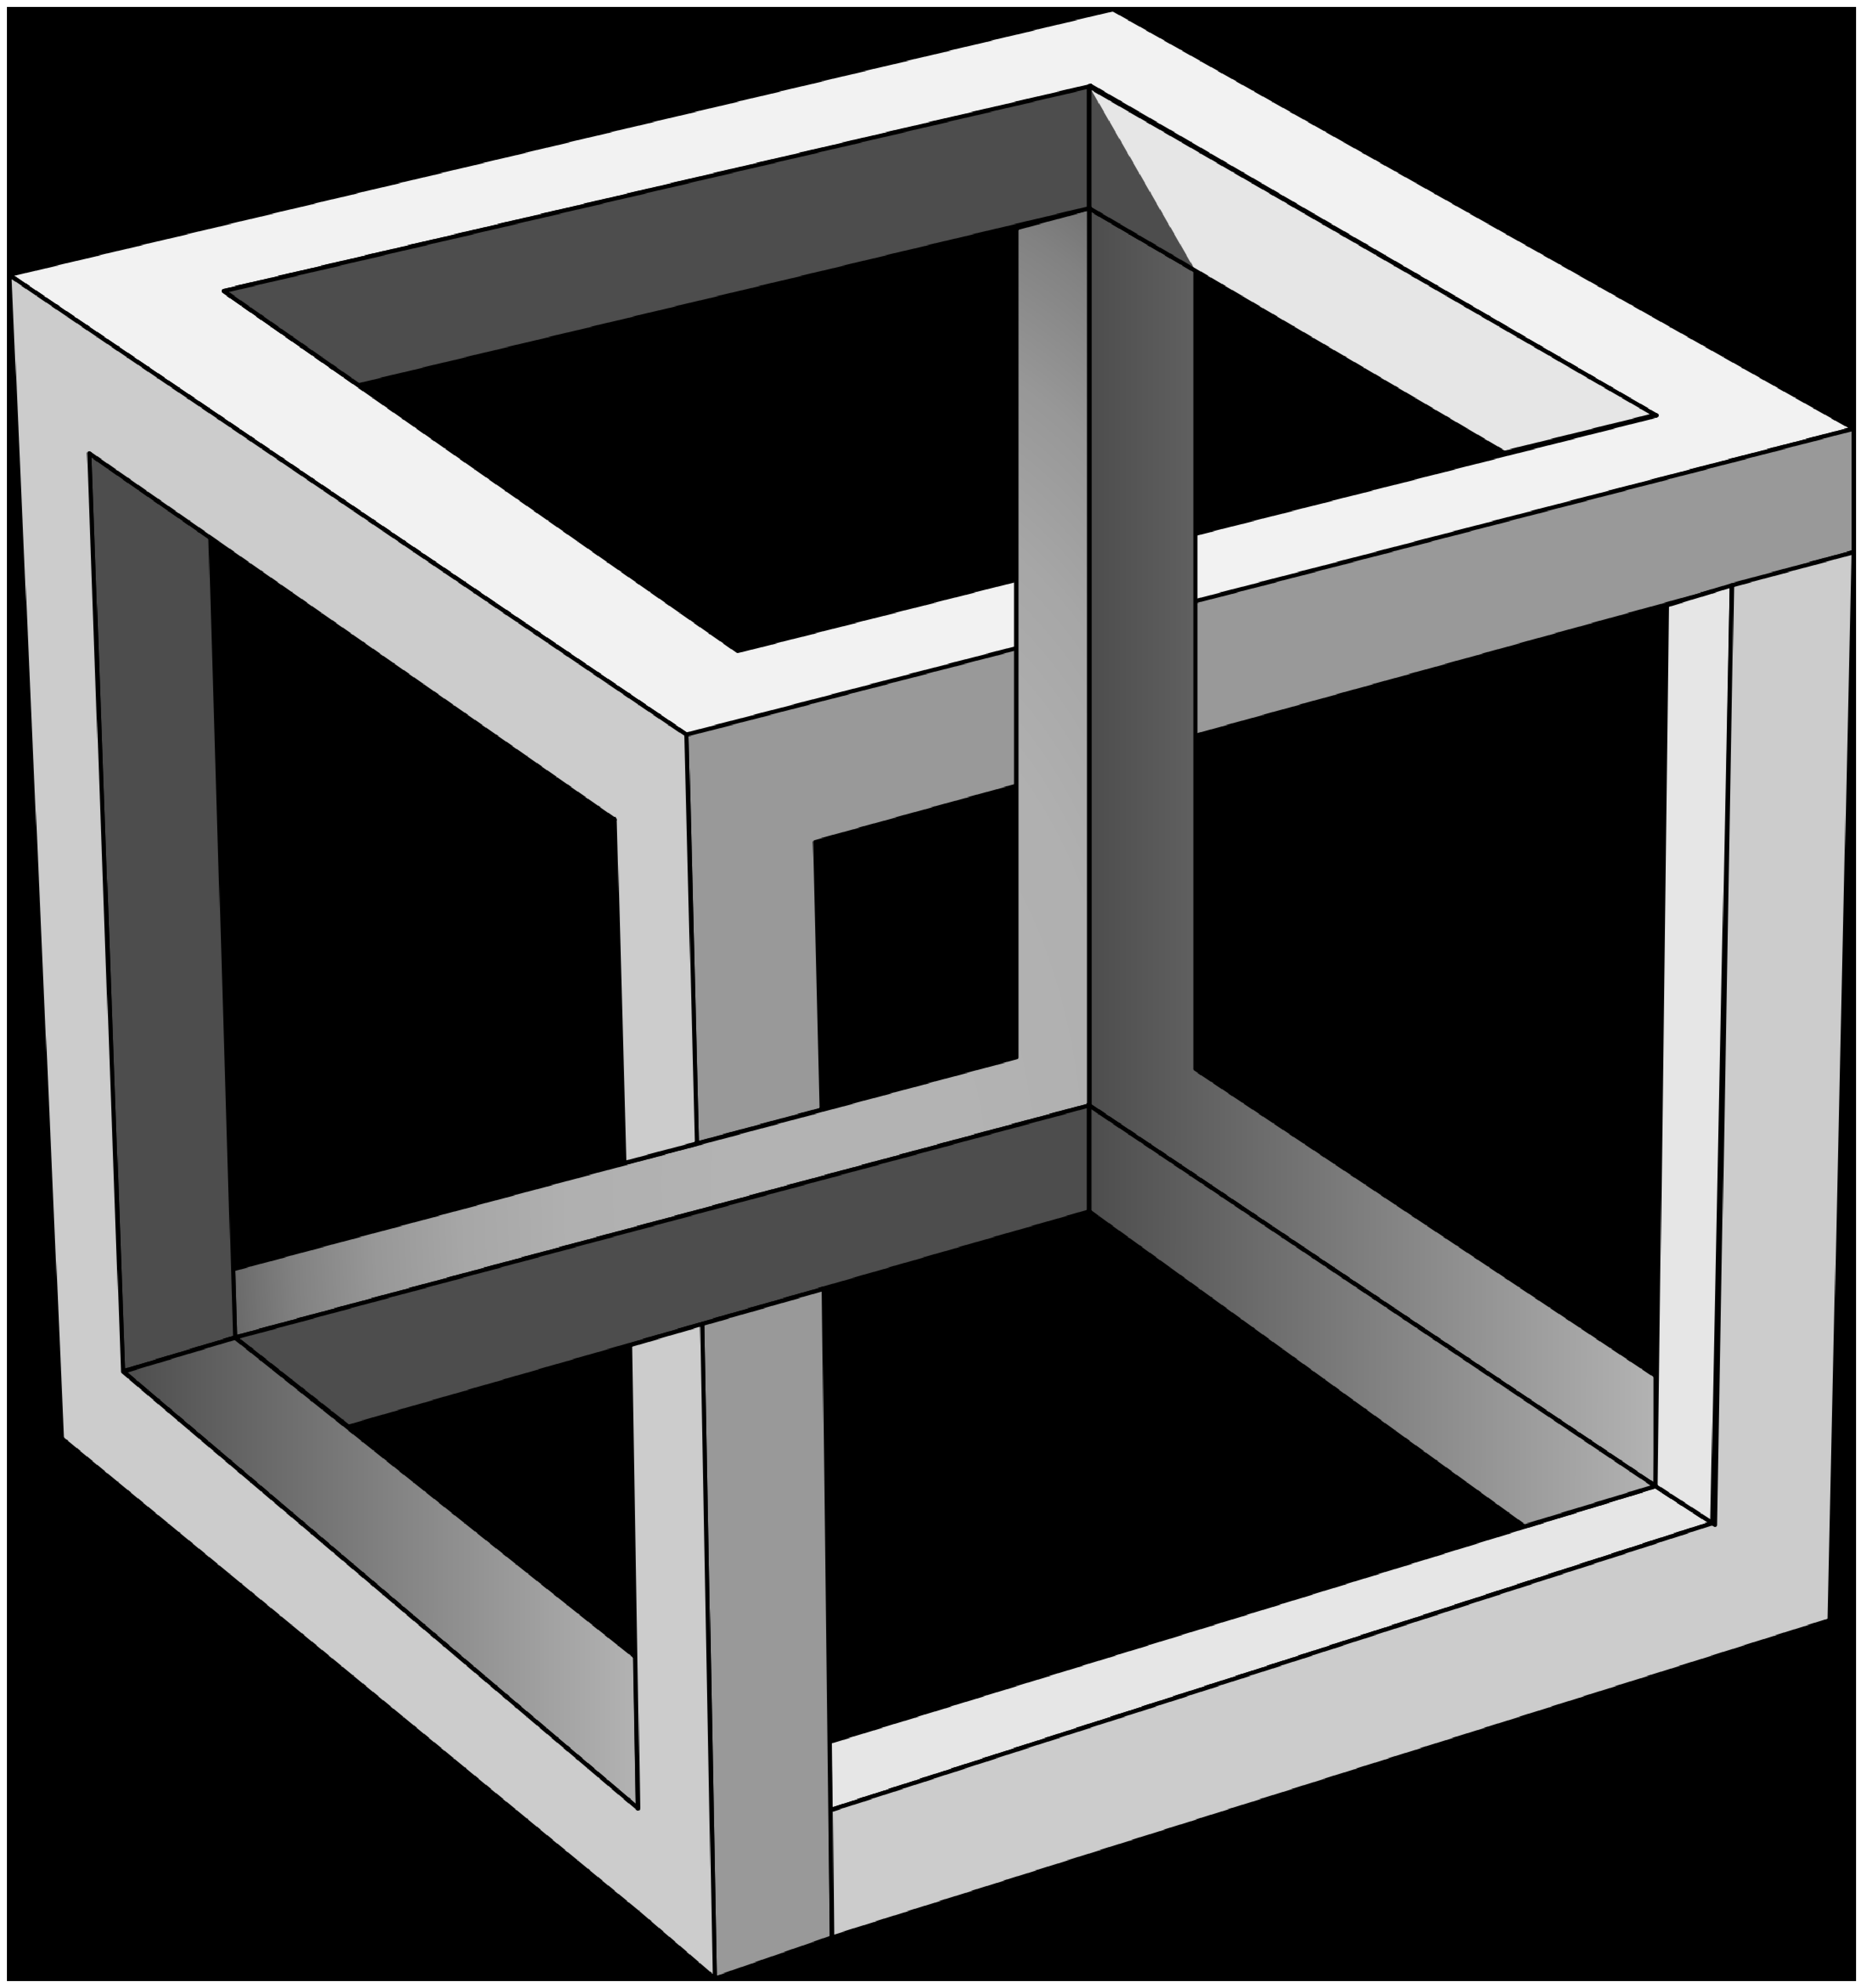
\includegraphics[scale=0.1]{Escher1.eps}
\end{center}
He aqui una gr'afica sencilla e interesante, enjoy!:
\begin{center}
	\setlength{\unitlength}{2pt}
	\begin{picture}(100,60)\thicklines
	{\color{gris}\graphpaper(0,0)(100,60)}
	\put(10,0){\line(2,3){40}}
	\put(20,0){\line(1,2){30}}
	\put(30,0){\line(1,3){20}}
	\put(40,0){\line(1,6){10}}
	\put(50,0){\line(0,1){60}}
	\put(60,0){\line(-1,6){10}}
	\put(70,0){\line(-1,3){20}}
	\put(80,0){\line(-1,2){30}}
	\put(90,0){\line(-2,3){40}}
	\put(10,0){\line(1,0){80}}
	\end{picture}
\end{center}

\end{document}